\chapter{Conclusion}
\label{cha:conclusion}

In this dissertation we developed a structure of projects that can interpret a \ac{XSD} document and use its contents to generate a fluent Java \ac{API} that allows to perform actions over the language defined in the \ac{XSD} document while enforcing most of the rules that exist in the \ac{XSD} syntax. The generated \ac{API} only reflects the structure described in the \ac{XSD} document, providing tools that allow any future usage to be defined according to the needs of the user. Upon testing the resulting solution we obtained better results than similar solutions while proving a solution with a fluent language, which should be intuitive even for people that never programmed in Java before, since it ends up being very similar to writing \ac{XML}.

\noindent
The main language definition used in order to test and develop this solution was the \ac{HTML}5 syntax, which generated the HtmlApi project, containing a set of classes reflecting all the elements and attributes present in the \ac{HTML} language. This HtmlApi project was then used by the HtmlFlow library in order to provide an \ac{API} that writes well formed \ac{HTML} documents. Other \ac{XSD} files were used to test the solution, such as the Android layouts definition file, which defines the existing \ac{XML} elements used to create visual layouts for the Android operating system and the attributes that each element contains.

\section{Future work}
\label{cha:futurework}

In the future there are already changes planed to the way that the \ac{API}s are generated. The current \ac{API}s generated by the present solution are built on a two step basis, first the user has to create the element tree and after finishing its creation the user can then visit the whole tree. Even though this solution provides security to the user and already provides better results than similar solutions there is an improved solution that should increase its performance in a significant way. The improved solution removes the two steps nature of the solution, avoiding storing elements in a data structure and then having to iterate that structure. An example of this new solution usage is shown in Listing \ref{lst:futuresolutionusage}. 

\bigskip

\lstset{language=java, morekeywords={Visitor, Html, body}}

\begin{minipage}{\linewidth}
\begin{lstlisting}[caption={Future Solution Usage 1}, label={lst:futuresolutionusage}]
Visitor visitor = new Visitor();
Html<Html> documentRoot = new Html<>(visitor);
documentRoot.body();
\end{lstlisting}
\end{minipage}

\noindent
With the root receiving the Visitor instance its possible to start calling the respective visit methods right away, as shown in class Html in Listing \ref{lst:futurehtmlclass} and Body in Listing \ref{lst:futurebodyclass}.

\bigskip

\lstset{language=java, morekeywords={Html, Visitor, visit, self, Body, getVisitor, SomeAttribute}}

\begin{minipage}{\linewidth}
\begin{lstlisting}[caption={Future Solution Html Class (Simplified)}, label={lst:futurehtmlclass}]
public class Html{
    private Visitor visitor;
	
    public Html(Visitor visitor){
        this.visitor = visitor;
        visitor.visit(this);
    }
	
    public Body body(){
        return new Body(this.self());
    }
    
    public Html someAttribute(String value){
        visitor.visit(new SomeAttribute(value));
        return this;
   }
}
\end{lstlisting}
\end{minipage}

\newpage

\lstset{language=java, morekeywords={Html, Visitor, visit, self, Body, getVisitor, SomeAttribute}}

\begin{minipage}{\linewidth}
\begin{lstlisting}[caption={Future Solution Body Class (Simplified)}, label={lst:futurebodyclass}]
public class Body{
    private Visitor visitor;

    public Body(Element parent){
        this.visitor = parent.getVisitor();
        this.visitor.visit(this);
    }	
}
\end{lstlisting}
\end{minipage}

\noindent
With this solution the overhead of using this solution is minimized, because as we can see the overhead of the code structure almost resumes itself to the overhead of instantiating classes. All the rules of the language are still enforced due to the way that the classes are organized and the usage keeps its fluent nature since the existent methods and its return type are unchanged. This also removes all the overhead of storing and iterating data from a data structure. Using this solution in the web world should improve the response times of servers in a very significant way since the solution can write to the response stream as soon as it executes the method code for adding an element, opposed to having to wait that the whole tree is built and only then iterated. 

\subsection{Early Results}

After implementing a first version of this improved solution, called HtmlApiFaster, we ran a few tests in order to evaluate its performance. The benchmark used was the same presented in Section \ref{sec:testingmetrics} with the spring-comparing-template-engines project. All the results presented below are presented without the respective Spring overhead, which was previously explained in Section \ref{sec:testingmetrics}.

\begin{multicols}{2}
10.000 requests, 10 threads:\\
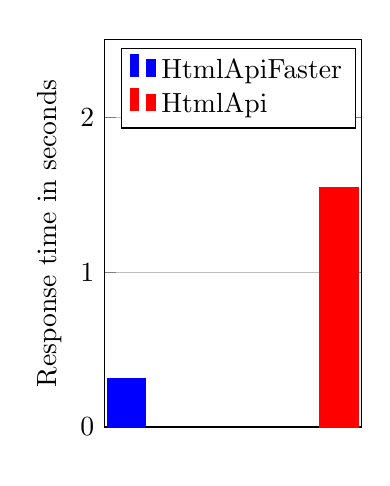
\begin{tikzpicture}
    \begin{axis}[
        width  = 0.4*\textwidth,
        height = 6.5cm,
        major x tick style = transparent,
        ybar=2*\pgflinewidth,
        bar width=14pt,
        ymajorgrids = true,
        ylabel = {Response time in seconds},
		symbolic x coords={HtmlApiFaster, HtmlApi},
        xticklabels = {},
        scaled y ticks = false,
        enlarge x limits=0.25,
        ymin=0,
        ymax=2.5,
        legend cell align=left,]
        
        \addplot[style={blue,fill=blue,mark=none}]
            coordinates {(HtmlApiFaster, 0.313)};
        \addplot[style={red,fill=red,mark=none}]
             coordinates {(HtmlApi, 1.547 )};
             
        \legend{HtmlApiFaster, HtmlApi}
    \end{axis}
\end{tikzpicture}
\columnbreak
\\
30.000 requests, 10 threads:\\
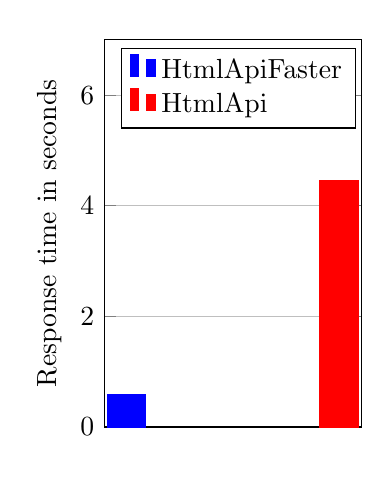
\begin{tikzpicture}
    \begin{axis}[
        width  = 0.4*\textwidth,
        height = 6.5cm,
        major x tick style = transparent,
        ybar=2*\pgflinewidth,
        bar width=14pt,
        ymajorgrids = true,
        ylabel = {Response time in seconds},
		symbolic x coords={HtmlApiFaster, HtmlApi},
        xticklabels = {},
        scaled y ticks = false,
        enlarge x limits=0.25,
        ymin=0,
        ymax=7,
        legend cell align=left,]
        
        \addplot[style={blue,fill=blue,mark=none}]
            coordinates {(HtmlApiFaster, 0.590)};
        \addplot[style={red,fill=red,mark=none}]
             coordinates {(HtmlApi, 4.450)};

        \legend{HtmlApiFaster, HtmlApi}
    \end{axis}
\end{tikzpicture}
\end{multicols}

\begin{multicols}{2}
30.000 requests, 25 threads:\\
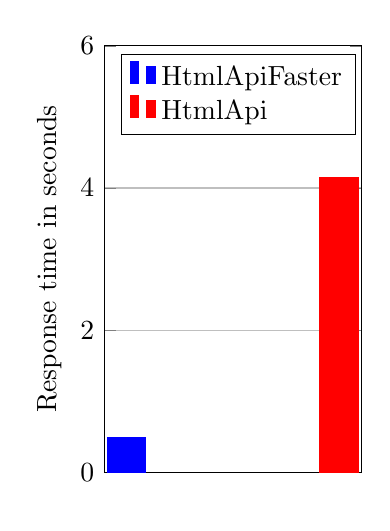
\begin{tikzpicture}
    \begin{axis}[
        width  = 0.4*\textwidth,
        height = 7cm,
        major x tick style = transparent,
        ybar=2*\pgflinewidth,
        bar width=14pt,
        ymajorgrids = true,
        ylabel = {Response time in seconds},
		symbolic x coords={HtmlApiFaster, HtmlApi},
        xticklabels = {},
        scaled y ticks = false,
        enlarge x limits=0.25,
        ymin=0,
        ymax=6,
        legend cell align=left,]
        
        \addplot[style={blue,fill=blue,mark=none}]
            coordinates {(HtmlApiFaster, 0.494)};
        \addplot[style={red,fill=red,mark=none}]
             coordinates {(HtmlApi, 4.151 )};
             
        \legend{HtmlApiFaster, HtmlApi}
    \end{axis}
\end{tikzpicture}
\columnbreak
\\
100.000 requests, 10 threads:\\
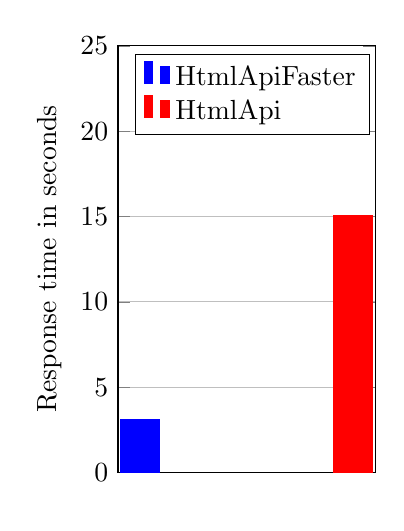
\begin{tikzpicture}
    \begin{axis}[
        width  = 0.4*\textwidth,
        height = 7cm,
        major x tick style = transparent,
        ybar=2*\pgflinewidth,
        bar width=14pt,
        ymajorgrids = true,
        ylabel = {Response time in seconds},
		symbolic x coords={HtmlApiFaster, HtmlApi},
        xticklabels = {},
        scaled y ticks = false,
        enlarge x limits=0.25,
        ymin=0,
        ymax=25,
        legend cell align=left,]
        
        \addplot[style={blue,fill=blue,mark=none}]
            coordinates {(HtmlApiFaster, 3.095)};
        \addplot[style={red,fill=red,mark=none}]
             coordinates {(HtmlApi, 15.049)};

        \legend{HtmlApiFaster, HtmlApi}
    \end{axis}
\end{tikzpicture}
\end{multicols}

As we can see the performance gains are very good, with the lowest gap being with the example using 100.000 requests where HtmlApiFaster is 4 times faster than HtmlApi. On the other hand the biggest difference is present in the example using 30.000 requests and 25 concurrent threads, where HtmlApiFaster is 8 times faster than HtmlApi which was already the better option when comparing to the template engines. These results are promising and the HtmlApiFaster will be further developed in order to deploy it as an alternative to HtmlApi.